% Options for packages loaded elsewhere
\PassOptionsToPackage{unicode}{hyperref}
\PassOptionsToPackage{hyphens}{url}
%
\documentclass[
]{article}
\usepackage{amsmath,amssymb}
\usepackage{iftex}
\ifPDFTeX
  \usepackage[T1]{fontenc}
  \usepackage[utf8]{inputenc}
  \usepackage{textcomp} % provide euro and other symbols
\else % if luatex or xetex
  \usepackage{unicode-math} % this also loads fontspec
  \defaultfontfeatures{Scale=MatchLowercase}
  \defaultfontfeatures[\rmfamily]{Ligatures=TeX,Scale=1}
\fi
\usepackage{lmodern}
\ifPDFTeX\else
  % xetex/luatex font selection
\fi
% Use upquote if available, for straight quotes in verbatim environments
\IfFileExists{upquote.sty}{\usepackage{upquote}}{}
\IfFileExists{microtype.sty}{% use microtype if available
  \usepackage[]{microtype}
  \UseMicrotypeSet[protrusion]{basicmath} % disable protrusion for tt fonts
}{}
\makeatletter
\@ifundefined{KOMAClassName}{% if non-KOMA class
  \IfFileExists{parskip.sty}{%
    \usepackage{parskip}
  }{% else
    \setlength{\parindent}{0pt}
    \setlength{\parskip}{6pt plus 2pt minus 1pt}}
}{% if KOMA class
  \KOMAoptions{parskip=half}}
\makeatother
\usepackage{xcolor}
\usepackage[margin=1in]{geometry}
\usepackage{color}
\usepackage{fancyvrb}
\newcommand{\VerbBar}{|}
\newcommand{\VERB}{\Verb[commandchars=\\\{\}]}
\DefineVerbatimEnvironment{Highlighting}{Verbatim}{commandchars=\\\{\}}
% Add ',fontsize=\small' for more characters per line
\usepackage{framed}
\definecolor{shadecolor}{RGB}{248,248,248}
\newenvironment{Shaded}{\begin{snugshade}}{\end{snugshade}}
\newcommand{\AlertTok}[1]{\textcolor[rgb]{0.94,0.16,0.16}{#1}}
\newcommand{\AnnotationTok}[1]{\textcolor[rgb]{0.56,0.35,0.01}{\textbf{\textit{#1}}}}
\newcommand{\AttributeTok}[1]{\textcolor[rgb]{0.13,0.29,0.53}{#1}}
\newcommand{\BaseNTok}[1]{\textcolor[rgb]{0.00,0.00,0.81}{#1}}
\newcommand{\BuiltInTok}[1]{#1}
\newcommand{\CharTok}[1]{\textcolor[rgb]{0.31,0.60,0.02}{#1}}
\newcommand{\CommentTok}[1]{\textcolor[rgb]{0.56,0.35,0.01}{\textit{#1}}}
\newcommand{\CommentVarTok}[1]{\textcolor[rgb]{0.56,0.35,0.01}{\textbf{\textit{#1}}}}
\newcommand{\ConstantTok}[1]{\textcolor[rgb]{0.56,0.35,0.01}{#1}}
\newcommand{\ControlFlowTok}[1]{\textcolor[rgb]{0.13,0.29,0.53}{\textbf{#1}}}
\newcommand{\DataTypeTok}[1]{\textcolor[rgb]{0.13,0.29,0.53}{#1}}
\newcommand{\DecValTok}[1]{\textcolor[rgb]{0.00,0.00,0.81}{#1}}
\newcommand{\DocumentationTok}[1]{\textcolor[rgb]{0.56,0.35,0.01}{\textbf{\textit{#1}}}}
\newcommand{\ErrorTok}[1]{\textcolor[rgb]{0.64,0.00,0.00}{\textbf{#1}}}
\newcommand{\ExtensionTok}[1]{#1}
\newcommand{\FloatTok}[1]{\textcolor[rgb]{0.00,0.00,0.81}{#1}}
\newcommand{\FunctionTok}[1]{\textcolor[rgb]{0.13,0.29,0.53}{\textbf{#1}}}
\newcommand{\ImportTok}[1]{#1}
\newcommand{\InformationTok}[1]{\textcolor[rgb]{0.56,0.35,0.01}{\textbf{\textit{#1}}}}
\newcommand{\KeywordTok}[1]{\textcolor[rgb]{0.13,0.29,0.53}{\textbf{#1}}}
\newcommand{\NormalTok}[1]{#1}
\newcommand{\OperatorTok}[1]{\textcolor[rgb]{0.81,0.36,0.00}{\textbf{#1}}}
\newcommand{\OtherTok}[1]{\textcolor[rgb]{0.56,0.35,0.01}{#1}}
\newcommand{\PreprocessorTok}[1]{\textcolor[rgb]{0.56,0.35,0.01}{\textit{#1}}}
\newcommand{\RegionMarkerTok}[1]{#1}
\newcommand{\SpecialCharTok}[1]{\textcolor[rgb]{0.81,0.36,0.00}{\textbf{#1}}}
\newcommand{\SpecialStringTok}[1]{\textcolor[rgb]{0.31,0.60,0.02}{#1}}
\newcommand{\StringTok}[1]{\textcolor[rgb]{0.31,0.60,0.02}{#1}}
\newcommand{\VariableTok}[1]{\textcolor[rgb]{0.00,0.00,0.00}{#1}}
\newcommand{\VerbatimStringTok}[1]{\textcolor[rgb]{0.31,0.60,0.02}{#1}}
\newcommand{\WarningTok}[1]{\textcolor[rgb]{0.56,0.35,0.01}{\textbf{\textit{#1}}}}
\usepackage{graphicx}
\makeatletter
\def\maxwidth{\ifdim\Gin@nat@width>\linewidth\linewidth\else\Gin@nat@width\fi}
\def\maxheight{\ifdim\Gin@nat@height>\textheight\textheight\else\Gin@nat@height\fi}
\makeatother
% Scale images if necessary, so that they will not overflow the page
% margins by default, and it is still possible to overwrite the defaults
% using explicit options in \includegraphics[width, height, ...]{}
\setkeys{Gin}{width=\maxwidth,height=\maxheight,keepaspectratio}
% Set default figure placement to htbp
\makeatletter
\def\fps@figure{htbp}
\makeatother
\setlength{\emergencystretch}{3em} % prevent overfull lines
\providecommand{\tightlist}{%
  \setlength{\itemsep}{0pt}\setlength{\parskip}{0pt}}
\setcounter{secnumdepth}{-\maxdimen} % remove section numbering
\ifLuaTeX
  \usepackage{selnolig}  % disable illegal ligatures
\fi
\IfFileExists{bookmark.sty}{\usepackage{bookmark}}{\usepackage{hyperref}}
\IfFileExists{xurl.sty}{\usepackage{xurl}}{} % add URL line breaks if available
\urlstyle{same}
\hypersetup{
  pdftitle={Regression\_model\_mtcars\_pdf},
  pdfauthor={Suhas P K},
  hidelinks,
  pdfcreator={LaTeX via pandoc}}

\title{Regression\_model\_mtcars\_pdf}
\author{Suhas P K}
\date{2023-07-17}

\begin{document}
\maketitle

\hypertarget{introduction}{%
\section{Introduction}\label{introduction}}

\textbf{Motor Trend} is a magazine about the automobile industry. In
this analysis, a data set having information of car collection is
explored to understand the relationship between \textbf{miles per
gallon} and \textbf{transmission type}.\\
The data set is available from the CRAN repository.\\

\hypertarget{libraries-used.}{%
\subsection{Libraries used.}\label{libraries-used.}}

\begin{Shaded}
\begin{Highlighting}[]
\FunctionTok{library}\NormalTok{(tinytex)}
\FunctionTok{library}\NormalTok{(ggplot2)}
\FunctionTok{library}\NormalTok{(ggdark)}
\end{Highlighting}
\end{Shaded}

\hypertarget{reading-the-data-set.}{%
\subsection{Reading the data set.}\label{reading-the-data-set.}}

\begin{Shaded}
\begin{Highlighting}[]
\FunctionTok{data}\NormalTok{(mtcars)}
\end{Highlighting}
\end{Shaded}

\hypertarget{basics-checking-of-the-data-set.}{%
\subsubsection{Basics checking of the data
set.}\label{basics-checking-of-the-data-set.}}

\begin{Shaded}
\begin{Highlighting}[]
\FunctionTok{summary}\NormalTok{(mtcars)}
\end{Highlighting}
\end{Shaded}

\begin{verbatim}
##       mpg             cyl             disp             hp       
##  Min.   :10.40   Min.   :4.000   Min.   : 71.1   Min.   : 52.0  
##  1st Qu.:15.43   1st Qu.:4.000   1st Qu.:120.8   1st Qu.: 96.5  
##  Median :19.20   Median :6.000   Median :196.3   Median :123.0  
##  Mean   :20.09   Mean   :6.188   Mean   :230.7   Mean   :146.7  
##  3rd Qu.:22.80   3rd Qu.:8.000   3rd Qu.:326.0   3rd Qu.:180.0  
##  Max.   :33.90   Max.   :8.000   Max.   :472.0   Max.   :335.0  
##       drat             wt             qsec             vs        
##  Min.   :2.760   Min.   :1.513   Min.   :14.50   Min.   :0.0000  
##  1st Qu.:3.080   1st Qu.:2.581   1st Qu.:16.89   1st Qu.:0.0000  
##  Median :3.695   Median :3.325   Median :17.71   Median :0.0000  
##  Mean   :3.597   Mean   :3.217   Mean   :17.85   Mean   :0.4375  
##  3rd Qu.:3.920   3rd Qu.:3.610   3rd Qu.:18.90   3rd Qu.:1.0000  
##  Max.   :4.930   Max.   :5.424   Max.   :22.90   Max.   :1.0000  
##        am              gear            carb      
##  Min.   :0.0000   Min.   :3.000   Min.   :1.000  
##  1st Qu.:0.0000   1st Qu.:3.000   1st Qu.:2.000  
##  Median :0.0000   Median :4.000   Median :2.000  
##  Mean   :0.4062   Mean   :3.688   Mean   :2.812  
##  3rd Qu.:1.0000   3rd Qu.:4.000   3rd Qu.:4.000  
##  Max.   :1.0000   Max.   :5.000   Max.   :8.000
\end{verbatim}

\hypertarget{check-the-structure-of-data-set.}{%
\subsubsection{Check the structure of data
set.}\label{check-the-structure-of-data-set.}}

\begin{Shaded}
\begin{Highlighting}[]
\FunctionTok{str}\NormalTok{(mtcars)}
\end{Highlighting}
\end{Shaded}

\begin{verbatim}
## 'data.frame':    32 obs. of  11 variables:
##  $ mpg : num  21 21 22.8 21.4 18.7 18.1 14.3 24.4 22.8 19.2 ...
##  $ cyl : num  6 6 4 6 8 6 8 4 4 6 ...
##  $ disp: num  160 160 108 258 360 ...
##  $ hp  : num  110 110 93 110 175 105 245 62 95 123 ...
##  $ drat: num  3.9 3.9 3.85 3.08 3.15 2.76 3.21 3.69 3.92 3.92 ...
##  $ wt  : num  2.62 2.88 2.32 3.21 3.44 ...
##  $ qsec: num  16.5 17 18.6 19.4 17 ...
##  $ vs  : num  0 0 1 1 0 1 0 1 1 1 ...
##  $ am  : num  1 1 1 0 0 0 0 0 0 0 ...
##  $ gear: num  4 4 4 3 3 3 3 4 4 4 ...
##  $ carb: num  4 4 1 1 2 1 4 2 2 4 ...
\end{verbatim}

\hypertarget{check-for-the-missing-data.}{%
\subsubsection{Check for the missing
data.}\label{check-for-the-missing-data.}}

\begin{Shaded}
\begin{Highlighting}[]
\FunctionTok{colSums}\NormalTok{(}\FunctionTok{is.na}\NormalTok{(mtcars))}
\end{Highlighting}
\end{Shaded}

\begin{verbatim}
##  mpg  cyl disp   hp drat   wt qsec   vs   am gear carb 
##    0    0    0    0    0    0    0    0    0    0    0
\end{verbatim}

There are no missing value.

\hypertarget{exploratory-data-analysis}{%
\subsection{Exploratory Data Analysis}\label{exploratory-data-analysis}}

\hypertarget{preliminary-analysis}{%
\subsubsection{Preliminary analysis}\label{preliminary-analysis}}

Understand the distribution of \textbf{miles per gallon} variable.

\begin{Shaded}
\begin{Highlighting}[]
\NormalTok{histplot }\OtherTok{\textless{}{-}} \FunctionTok{ggplot}\NormalTok{(}\AttributeTok{data =}\NormalTok{ mtcars,}
                   \FunctionTok{aes}\NormalTok{(}\AttributeTok{x =}\NormalTok{ mtcars}\SpecialCharTok{$}\NormalTok{mpg)) }\SpecialCharTok{+} \FunctionTok{geom\_histogram}\NormalTok{(}\AttributeTok{color =} \StringTok{"black"}\NormalTok{,}\AttributeTok{fill =} \StringTok{"lightgreen"}\NormalTok{) }\SpecialCharTok{+}
    \FunctionTok{xlab}\NormalTok{(}\StringTok{"miles per gallon"}\NormalTok{)}\SpecialCharTok{+}
    \FunctionTok{ggtitle}\NormalTok{(}\StringTok{"Histogram of Miles per gallon"}\NormalTok{)}\SpecialCharTok{+}
    \FunctionTok{dark\_theme\_light}\NormalTok{()}
\end{Highlighting}
\end{Shaded}

\begin{verbatim}
## Inverted geom defaults of fill and color/colour.
## To change them back, use invert_geom_defaults().
\end{verbatim}

\begin{Shaded}
\begin{Highlighting}[]
\NormalTok{histplot}
\end{Highlighting}
\end{Shaded}

\begin{verbatim}
## `stat_bin()` using `bins = 30`. Pick better value with `binwidth`.
\end{verbatim}

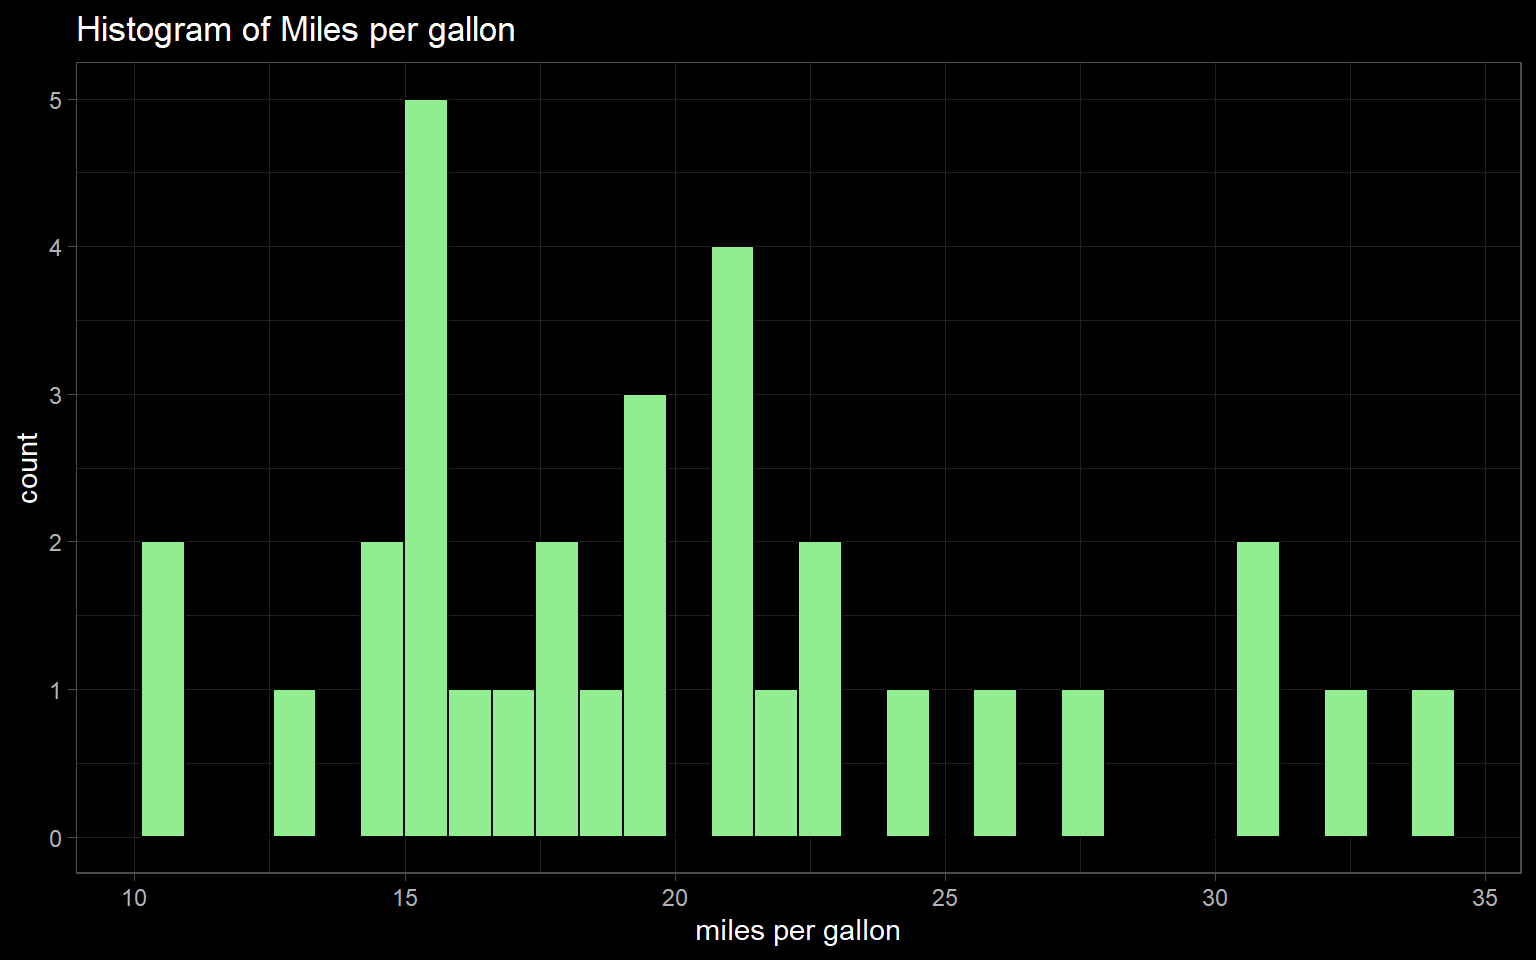
\includegraphics{Regression_model_mtcars_pdf_files/figure-latex/histogram of mpg-1.pdf}

Plotting a scatter plot based on the transmission type and mpg.

\begin{Shaded}
\begin{Highlighting}[]
\NormalTok{scttrplot }\OtherTok{\textless{}{-}} \FunctionTok{ggplot}\NormalTok{(}\AttributeTok{data =}\NormalTok{ mtcars,}
                    \FunctionTok{aes}\NormalTok{(}\AttributeTok{x =}\NormalTok{ am, }\AttributeTok{y =}\NormalTok{ mpg, }\AttributeTok{color =} \FunctionTok{factor}\NormalTok{(am)))}\SpecialCharTok{+} 
    \FunctionTok{geom\_point}\NormalTok{(}\AttributeTok{size =} \DecValTok{2}\NormalTok{)}\SpecialCharTok{+}\FunctionTok{geom\_smooth}\NormalTok{(}\AttributeTok{method=}\NormalTok{lm, }\AttributeTok{color =} \StringTok{"yellow"}\NormalTok{)}

\NormalTok{scttrplot }\SpecialCharTok{+}
    \FunctionTok{xlab}\NormalTok{(}\StringTok{"Transmission"}\NormalTok{)}\SpecialCharTok{+}
    \FunctionTok{ylab}\NormalTok{(}\StringTok{"miles per gallon"}\NormalTok{)}\SpecialCharTok{+}
    \FunctionTok{scale\_colour\_discrete}\NormalTok{(}
        \AttributeTok{name =} \StringTok{"Transmission"}\NormalTok{,}
        \AttributeTok{limits =} \FunctionTok{c}\NormalTok{(}\StringTok{"0"}\NormalTok{,}\StringTok{"1"}\NormalTok{),}
        \AttributeTok{labels =} \FunctionTok{c}\NormalTok{(}\StringTok{"Automatic"}\NormalTok{,}
                   \StringTok{"Manual"}\NormalTok{)}
\NormalTok{    ) }\SpecialCharTok{+} \FunctionTok{dark\_theme\_linedraw}\NormalTok{()}
\end{Highlighting}
\end{Shaded}

\begin{verbatim}
## `geom_smooth()` using formula = 'y ~ x'
\end{verbatim}

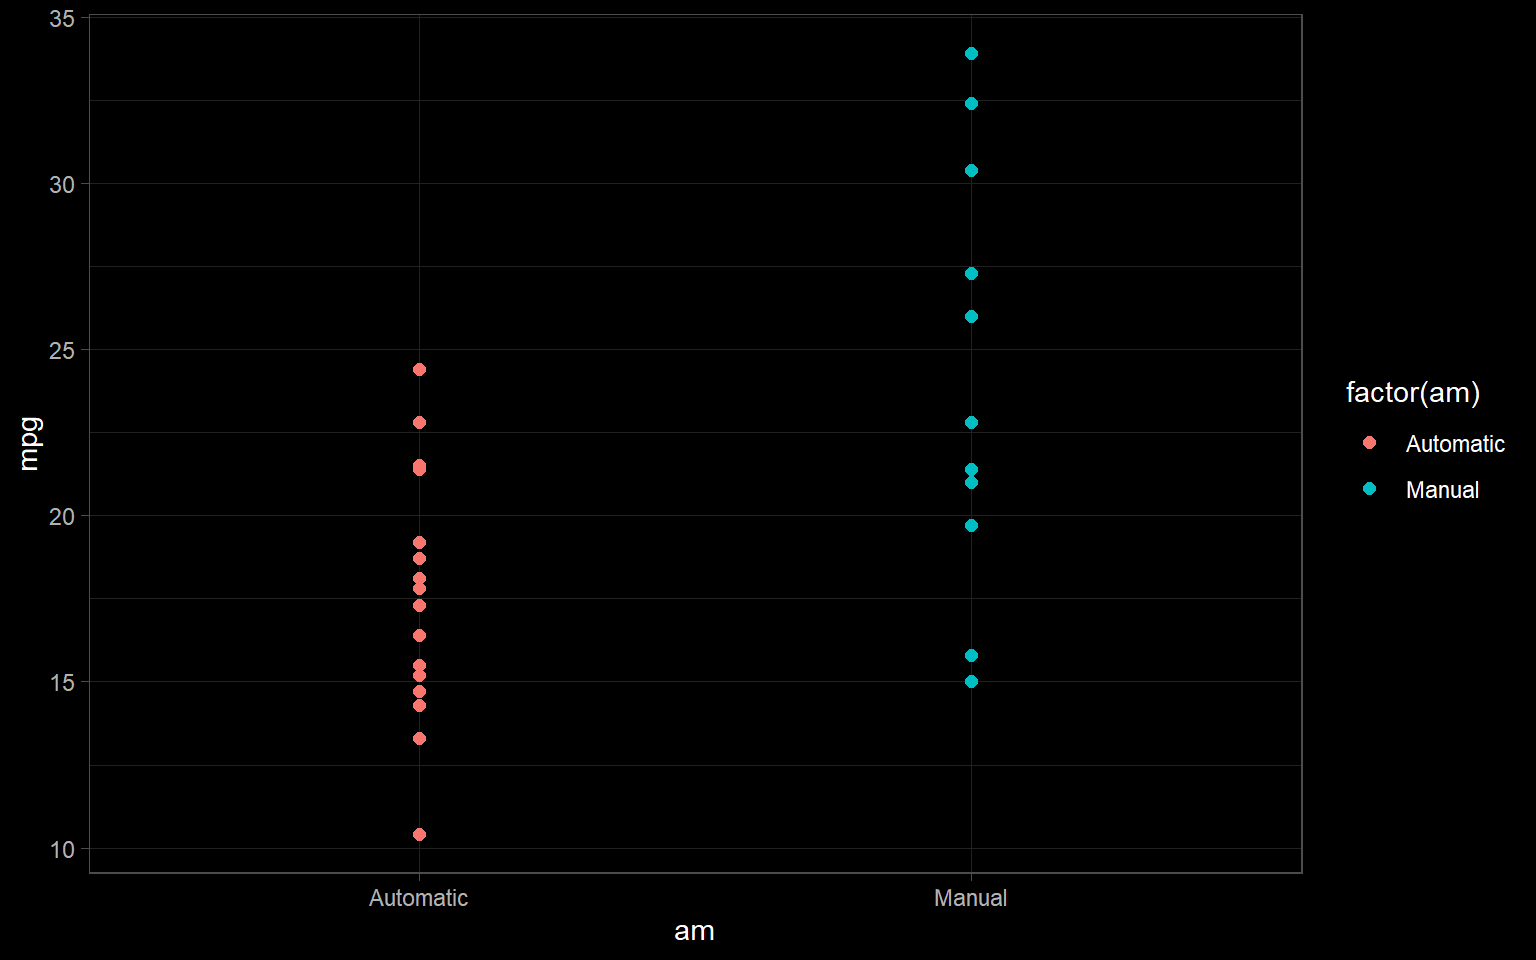
\includegraphics{Regression_model_mtcars_pdf_files/figure-latex/scatter plot-1.pdf}

Visualizing the `mpg' vs `transmission' using boxplot.

\begin{Shaded}
\begin{Highlighting}[]
\NormalTok{    bxplot }\OtherTok{\textless{}{-}} \FunctionTok{ggplot}\NormalTok{(mtcars, }\FunctionTok{aes}\NormalTok{(}\AttributeTok{x=}\FunctionTok{factor}\NormalTok{(am),}\AttributeTok{y =}\NormalTok{ mpg, }\AttributeTok{color =} \FunctionTok{factor}\NormalTok{(am)))}\SpecialCharTok{+}
    \FunctionTok{geom\_boxplot}\NormalTok{() }\SpecialCharTok{+}
    \FunctionTok{geom\_point}\NormalTok{(}\AttributeTok{stat =} \StringTok{"summary"}\NormalTok{,}
              \AttributeTok{fun =} \StringTok{"mean"}\NormalTok{,}
              \AttributeTok{color =} \StringTok{"white"}\NormalTok{, }\AttributeTok{label =} \StringTok{"mean"}\NormalTok{)}\SpecialCharTok{+}
    \FunctionTok{xlab}\NormalTok{(}\StringTok{"Transmission"}\NormalTok{)}\SpecialCharTok{+}
    \FunctionTok{ylab}\NormalTok{(}\StringTok{"Miles per gallon"}\NormalTok{)}
\end{Highlighting}
\end{Shaded}

\begin{verbatim}
## Warning in geom_point(stat = "summary", fun = "mean", color = "white", label =
## "mean"): Ignoring unknown parameters: `label`
\end{verbatim}

\begin{Shaded}
\begin{Highlighting}[]
\NormalTok{bxplot }\SpecialCharTok{+}
    \FunctionTok{scale\_colour\_discrete}\NormalTok{(}
    \AttributeTok{name =} \StringTok{"Tranmission"}\NormalTok{,}
    \AttributeTok{limits =} \FunctionTok{c}\NormalTok{(}\StringTok{"0"}\NormalTok{,}\StringTok{"1"}\NormalTok{),}
    \AttributeTok{labels =} \FunctionTok{c}\NormalTok{(}\StringTok{"Automatic"}\NormalTok{,}\StringTok{"Manual"}\NormalTok{)}
\NormalTok{) }\SpecialCharTok{+} \FunctionTok{dark\_theme\_light}\NormalTok{()}
\end{Highlighting}
\end{Shaded}

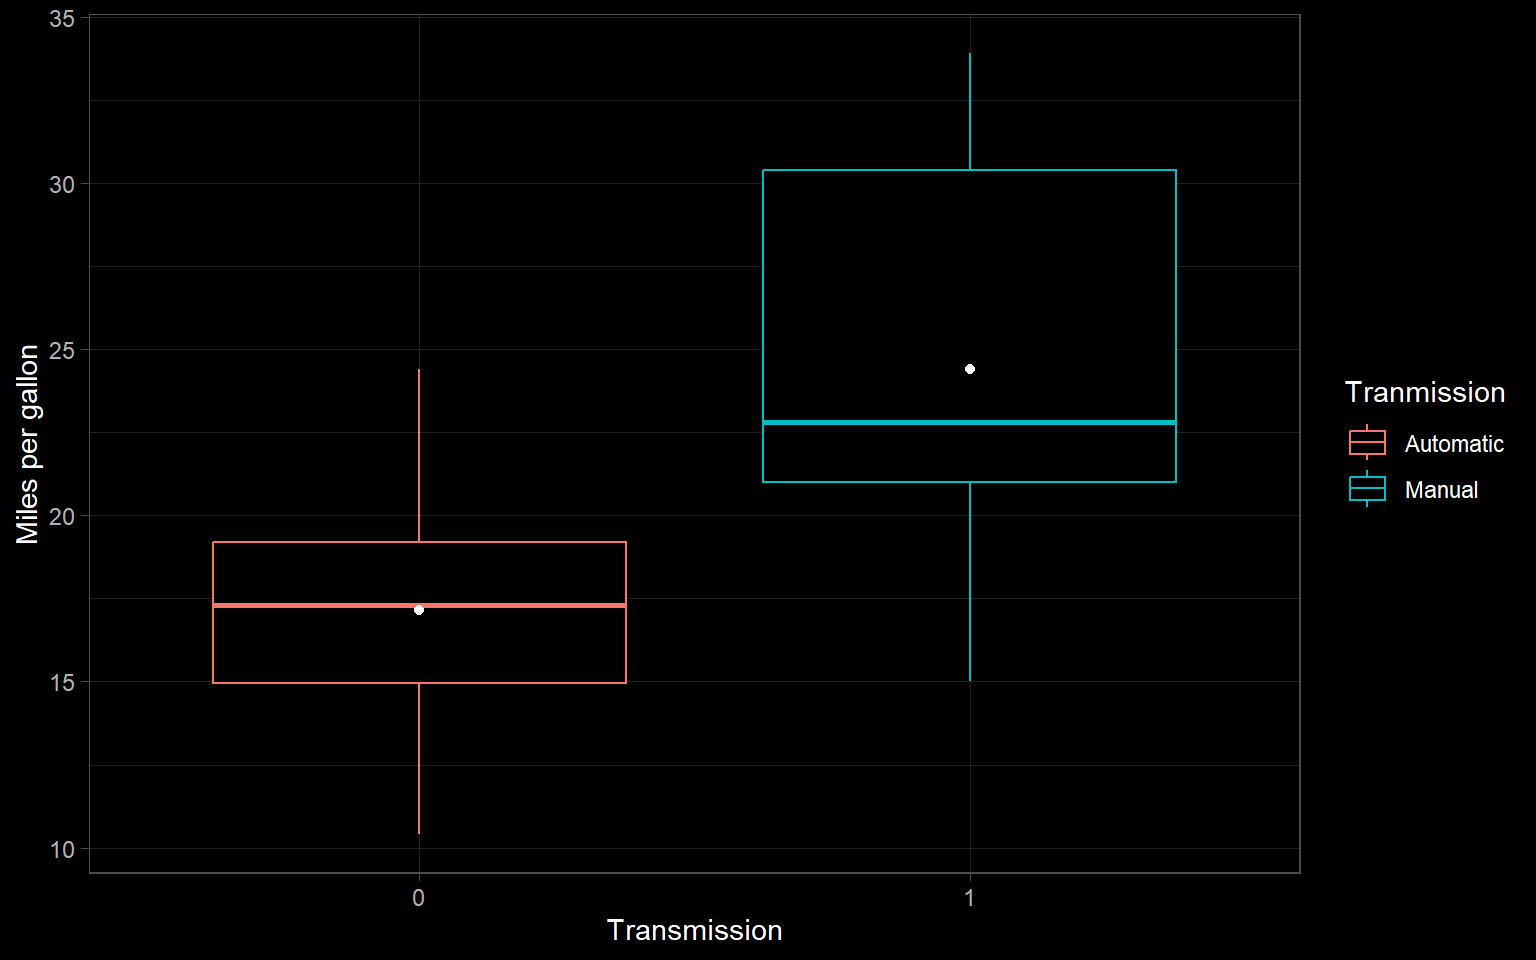
\includegraphics{Regression_model_mtcars_pdf_files/figure-latex/boxplot-1.pdf}
To understand better from the scatter plot, the mean value of mpg based
on the transmission type must be calculated. By far for this calculation
I will use this method.

\begin{Shaded}
\begin{Highlighting}[]
\NormalTok{mean\_am }\OtherTok{\textless{}{-}} \FunctionTok{with}\NormalTok{(mtcars,}
               \FunctionTok{tapply}\NormalTok{(mpg, am, mean))}
\NormalTok{mean\_am }
\end{Highlighting}
\end{Shaded}

\begin{verbatim}
##        0        1 
## 17.14737 24.39231
\end{verbatim}

Now take the difference between the median based on the transmission
type. With this we will get to know which transmission type has better
mpg.

\begin{Shaded}
\begin{Highlighting}[]
\NormalTok{mean\_am[}\DecValTok{2}\NormalTok{]}\SpecialCharTok{{-}}\NormalTok{mean\_am[}\DecValTok{1}\NormalTok{]}
\end{Highlighting}
\end{Shaded}

\begin{verbatim}
##        1 
## 7.244939
\end{verbatim}

In this case, the mean shows that, cars recorded with manual
transmission can travel 7.24 more miles per gallon on average than the
cars with automatic transmission.\\
Thus, manual transmission is better than the automatic.

\hypertarget{a-bit-advance-analysis}{%
\subsubsection{A bit advance analysis}\label{a-bit-advance-analysis}}

Performing \textbf{t-test} comparing the mean between the two
transmission groups.

\begin{Shaded}
\begin{Highlighting}[]
\NormalTok{am\_auto }\OtherTok{\textless{}{-}}\NormalTok{ mtcars}\SpecialCharTok{$}\NormalTok{mpg[mtcars}\SpecialCharTok{$}\NormalTok{am }\SpecialCharTok{==} \DecValTok{0}\NormalTok{]}
\NormalTok{am\_man }\OtherTok{\textless{}{-}}\NormalTok{ mtcars}\SpecialCharTok{$}\NormalTok{mpg[mtcars}\SpecialCharTok{$}\NormalTok{am }\SpecialCharTok{==} \DecValTok{1}\NormalTok{]}
\FunctionTok{t.test}\NormalTok{(}
\NormalTok{    am\_auto, am\_man,}
    \AttributeTok{paired =} \ConstantTok{FALSE}\NormalTok{,}
    \AttributeTok{alternative =} \StringTok{"two.sided"}\NormalTok{,}
    \AttributeTok{var.equal =} \ConstantTok{FALSE}
\NormalTok{)}
\end{Highlighting}
\end{Shaded}

\begin{verbatim}
## 
##  Welch Two Sample t-test
## 
## data:  am_auto and am_man
## t = -3.7671, df = 18.332, p-value = 0.001374
## alternative hypothesis: true difference in means is not equal to 0
## 95 percent confidence interval:
##  -11.280194  -3.209684
## sample estimates:
## mean of x mean of y 
##  17.14737  24.39231
\end{verbatim}

The confidence interval (95\%) does not contain zero (-11.28,-3.21) and
p-value is greater then 0.005. Then, it can conclude that the average
consumption, in miles per gallon, with automatic transmission is higher
than the manual transmission. In this case, the mean analysis, it is
possible to quantify the MPG difference between automatic and manual
transmissions: 7.24 mpg greater, subtracting means.

\hypertarget{regression-analysis}{%
\subsubsection{Regression analysis}\label{regression-analysis}}

\textbf{Single Model linear model} The analysis is made to compare
results from the \textbf{mean analysis}. The null hypothesis is that the
difference between mean of \textbf{mpg} and \textbf{am} is zero.

\begin{Shaded}
\begin{Highlighting}[]
\NormalTok{single\_model }\OtherTok{\textless{}{-}} 
    \FunctionTok{lm}\NormalTok{(mtcars}\SpecialCharTok{$}\NormalTok{mpg }\SpecialCharTok{\textasciitilde{}}\NormalTok{ mtcars}\SpecialCharTok{$}\NormalTok{am)}
\FunctionTok{summary}\NormalTok{(single\_model)}\SpecialCharTok{$}\NormalTok{coefficients}
\end{Highlighting}
\end{Shaded}

\begin{verbatim}
##              Estimate Std. Error   t value     Pr(>|t|)
## (Intercept) 17.147368   1.124603 15.247492 1.133983e-15
## mtcars$am    7.244939   1.764422  4.106127 2.850207e-04
\end{verbatim}

The results show us that the p-value of the slope is less than 0.005.
Then, it can reject the null hypothesis, and the results of the
exploratory analysis were confirmed: automatic transmission results are
7.245 miles per gallon greater. If the slope is greater than zero,
manual transmission is better than the automatic one.

\hypertarget{multivariable-analysis.}{%
\subsubsection{Multivariable analysis.}\label{multivariable-analysis.}}

\begin{Shaded}
\begin{Highlighting}[]
\FunctionTok{require}\NormalTok{(MASS)}
\end{Highlighting}
\end{Shaded}

\begin{verbatim}
## Loading required package: MASS
\end{verbatim}

\begin{Shaded}
\begin{Highlighting}[]
\NormalTok{multi\_model }\OtherTok{\textless{}{-}} \FunctionTok{stepAIC}\NormalTok{(}
    \FunctionTok{lm}\NormalTok{(mpg}\SpecialCharTok{\textasciitilde{}}\NormalTok{. , }\AttributeTok{data =}\NormalTok{ mtcars),}
    \AttributeTok{direction =} \StringTok{"both"}\NormalTok{,}
    \AttributeTok{trace =} \ConstantTok{FALSE}
\NormalTok{)}
\NormalTok{multi\_model}\SpecialCharTok{$}\NormalTok{anova}
\end{Highlighting}
\end{Shaded}

\begin{verbatim}
## Stepwise Model Path 
## Analysis of Deviance Table
## 
## Initial Model:
## mpg ~ cyl + disp + hp + drat + wt + qsec + vs + am + gear + carb
## 
## Final Model:
## mpg ~ wt + qsec + am
## 
## 
##     Step Df   Deviance Resid. Df Resid. Dev      AIC
## 1                             21   147.4944 70.89774
## 2  - cyl  1 0.07987121        22   147.5743 68.91507
## 3   - vs  1 0.26852280        23   147.8428 66.97324
## 4 - carb  1 0.68546077        24   148.5283 65.12126
## 5 - gear  1 1.56497053        25   150.0933 63.45667
## 6 - drat  1 3.34455117        26   153.4378 62.16190
## 7 - disp  1 6.62865369        27   160.0665 61.51530
## 8   - hp  1 9.21946935        28   169.2859 61.30730
\end{verbatim}

The \textbf{best model} indicated by the automated analysis consists of
the variables \textbf{wt}, \textbf{qsec}, \textbf{am} and \textbf{mpg}
as the outcome.

\begin{Shaded}
\begin{Highlighting}[]
\NormalTok{final\_model }\OtherTok{\textless{}{-}} \FunctionTok{lm}\NormalTok{(mtcars}\SpecialCharTok{$}\NormalTok{mpg }\SpecialCharTok{\textasciitilde{}}
\NormalTok{                      mtcars}\SpecialCharTok{$}\NormalTok{wt }\SpecialCharTok{+}\NormalTok{ mtcars}\SpecialCharTok{$}\NormalTok{qsec }\SpecialCharTok{+}\NormalTok{ mtcars}\SpecialCharTok{$}\NormalTok{am)}
\FunctionTok{summary}\NormalTok{(final\_model)}\SpecialCharTok{$}\NormalTok{coefficients}
\end{Highlighting}
\end{Shaded}

\begin{verbatim}
##              Estimate Std. Error   t value     Pr(>|t|)
## (Intercept)  9.617781  6.9595930  1.381946 1.779152e-01
## mtcars$wt   -3.916504  0.7112016 -5.506882 6.952711e-06
## mtcars$qsec  1.225886  0.2886696  4.246676 2.161737e-04
## mtcars$am    2.935837  1.4109045  2.080819 4.671551e-02
\end{verbatim}

Then, the regression equation is
\(mpg = 9.618 -3.917 wt + 1.226 qsec + 1.4109 am\) . It is assumed that
\(Errors = 0\). As the two-sided p-value for the \textbf{am} coefficient
is 0.04672, smaller than 0.05, it can we reject the null
hypothesis.Looking at the plots,

\begin{Shaded}
\begin{Highlighting}[]
\FunctionTok{par}\NormalTok{(}\AttributeTok{mfrow =} \FunctionTok{c}\NormalTok{(}\DecValTok{2}\NormalTok{,}\DecValTok{2}\NormalTok{))}
\FunctionTok{plot}\NormalTok{(final\_model)}
\end{Highlighting}
\end{Shaded}

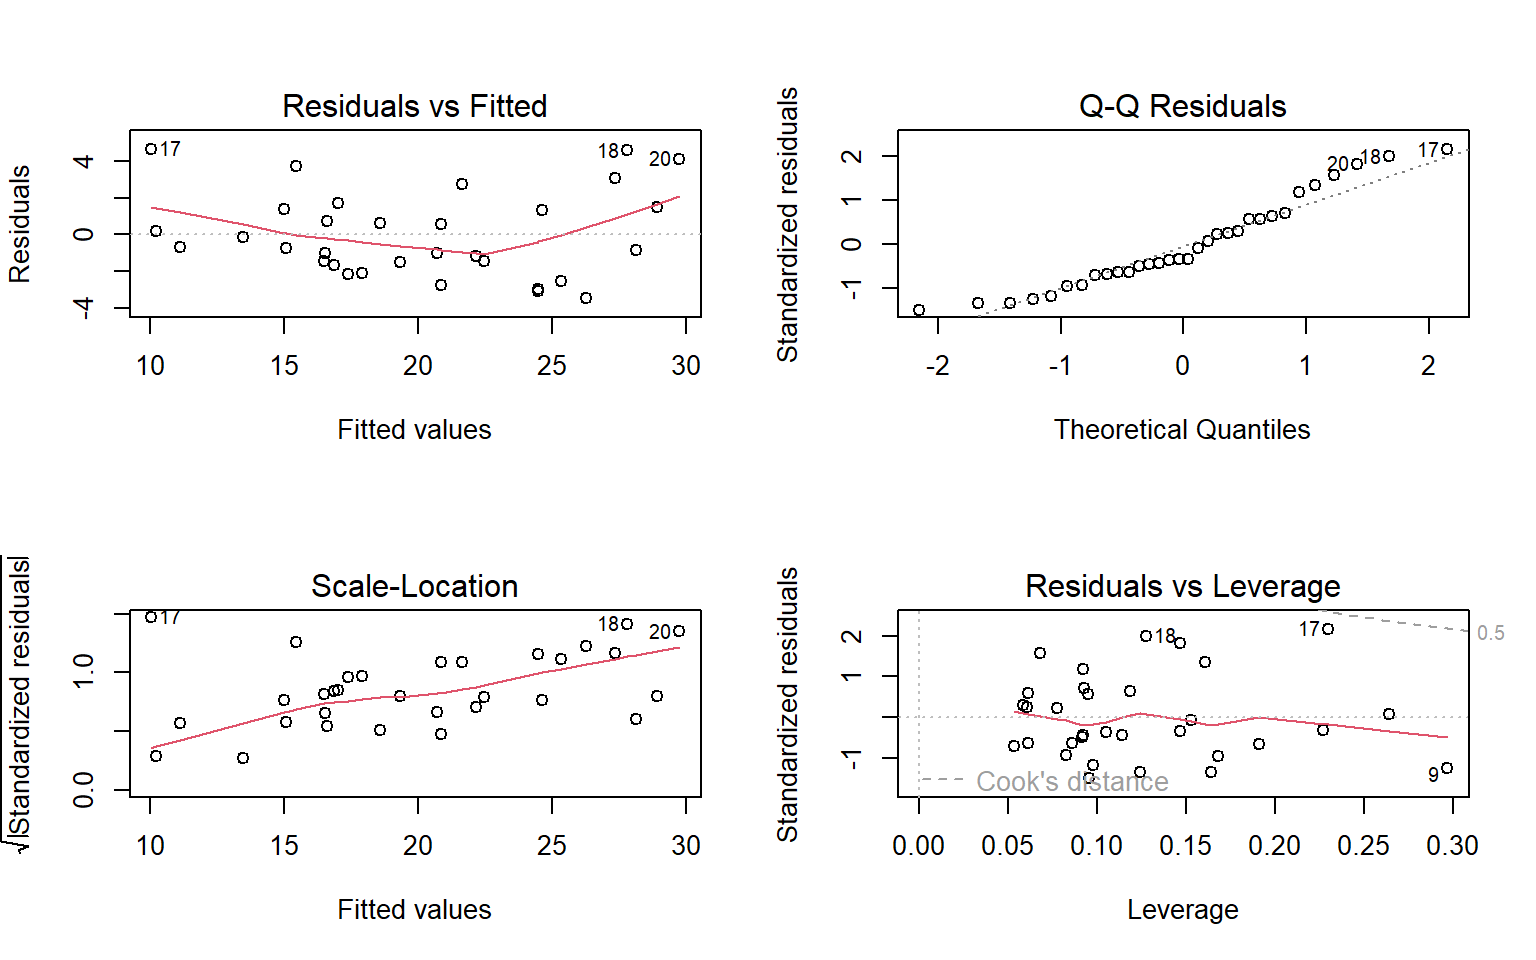
\includegraphics{Regression_model_mtcars_pdf_files/figure-latex/residual plot-1.pdf}
Final Model Residuals , the visual analysis show us that the behavior of
the best model is adequate considering normal residuals and constant
variability. The leverage is within reasonable upper limit.

\hypertarget{conclusion}{%
\subsection{Conclusion}\label{conclusion}}

\begin{itemize}
\tightlist
\item
  Manual transmission is better than the automatic.
\item
  Cars analyzed with manual transmission can travel 7.24 more miles per
  gallon on average than the cars with automatic transmission.
\item
  There is a correlation between mpg and transmission, but other
  variables should also be considered, as qsec and wt, beyond the type
  of transmission.
\item
  The obtained regression equation is \textbf{mpg = 9.618 -3.917 wt +
  1.226 qsec + 1.4109 am} . Then, for the same weight (wt) and quarter
  mile time (qsec),manual transmission cars get 1.4109 miles per gallon
  more than automatic transmission cars.
\end{itemize}

\end{document}
